\documentclass[border=10pt]{standalone}
\usepackage{tikz}
\usetikzlibrary{shapes, arrows.meta, positioning, fit}

\definecolor{hostblue}{HTML}{4A90D9}
\definecolor{espsoft}{HTML}{4A904A}
\definecolor{actred}{HTML}{D94A4A}
\definecolor{warn}{HTML}{D4A017}

\tikzset{
    layer/.style={rectangle, draw, minimum width=9cm, minimum height=1.4cm, align=center, font=\small},
    check/.style={rectangle, draw, fill=white, minimum width=2cm, minimum height=0.5cm, align=center, font=\scriptsize},
    arr/.style={-{Stealth[length=2mm]}, thick},
}

\begin{document}
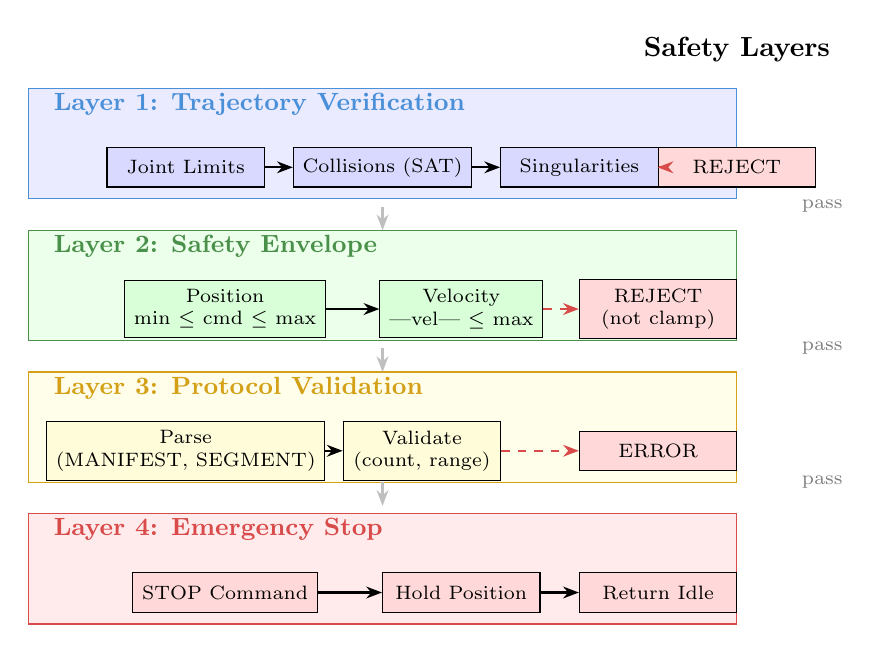
\begin{tikzpicture}[node distance=0.4cm]

\node[font=\bfseries] at (4.5, 0.2) {Safety Layers};

% ── Layer 1 ──
\node[layer, fill=blue!8, draw=hostblue] (l1) at (0, -1) {};
\node[font=\small\bfseries, hostblue, anchor=west] at (-4.3, -0.5) {Layer 1: Trajectory Verification};
\node[check, fill=blue!15] (jl) at (-2.5, -1.3) {Joint Limits};
\node[check, fill=blue!15] (col) at (0, -1.3) {Collisions (SAT)};
\node[check, fill=blue!15] (sing) at (2.5, -1.3) {Singularities};
\node[check, fill=red!15] (rej1) at (4.5, -1.3) {REJECT};

\draw[arr] (jl) -- (col);
\draw[arr] (col) -- (sing);
\draw[arr, dashed, actred] (sing) -- (rej1);

% ── Layer 2 ──
\node[layer, fill=green!8, draw=espsoft] (l2) at (0, -2.8) {};
\node[font=\small\bfseries, espsoft, anchor=west] at (-4.3, -2.3) {Layer 2: Safety Envelope};
\node[check, fill=green!15] (pos) at (-2, -3.1) {Position\\min $\le$ cmd $\le$ max};
\node[check, fill=green!15] (vel) at (1, -3.1) {Velocity\\|vel| $\le$ max};
\node[check, fill=red!15] (rej2) at (3.5, -3.1) {REJECT\\(not clamp)};

\draw[arr] (pos) -- (vel);
\draw[arr, dashed, actred] (vel) -- (rej2);

% ── Layer 3 ──
\node[layer, fill=yellow!8, draw=warn] (l3) at (0, -4.6) {};
\node[font=\small\bfseries, warn, anchor=west] at (-4.3, -4.1) {Layer 3: Protocol Validation};
\node[check, fill=yellow!15] (pars) at (-2.5, -4.9) {Parse\\(MANIFEST, SEGMENT)};
\node[check, fill=yellow!15] (val3) at (0.5, -4.9) {Validate\\(count, range)};
\node[check, fill=red!15] (rej3) at (3.5, -4.9) {ERROR};

\draw[arr] (pars) -- (val3);
\draw[arr, dashed, actred] (val3) -- (rej3);

% ── Layer 4 ──
\node[layer, fill=red!8, draw=actred] (l4) at (0, -6.4) {};
\node[font=\small\bfseries, actred, anchor=west] at (-4.3, -5.9) {Layer 4: Emergency Stop};
\node[check, fill=red!15] (stop) at (-2, -6.7) {STOP Command};
\node[check, fill=red!15] (hold) at (1, -6.7) {Hold Position};
\node[check, fill=red!15] (reset) at (3.5, -6.7) {Return Idle};

\draw[arr] (stop) -- (hold);
\draw[arr] (hold) -- (reset);

% ── Vertical flow ──
\draw[arr, gray!50] (0, -1.8) -- (0, -2.1);
\draw[arr, gray!50] (0, -3.6) -- (0, -3.9);
\draw[arr, gray!50] (0, -5.3) -- (0, -5.6);

\node[font=\scriptsize, gray, anchor=west] at (5.2, -1.8) {pass};
\node[font=\scriptsize, gray, anchor=west] at (5.2, -3.6) {pass};
\node[font=\scriptsize, gray, anchor=west] at (5.2, -5.3) {pass};

\end{tikzpicture}
\end{document}
